% !TEX TS-program = pdflatex
% !TEX encoding = UTF-8 Unicode

% This is a simple template for a LaTeX document using the "article" class.
% See "book", "report", "letter" for other types of document.

\documentclass[11pt]{article} % use larger type; default would be 10pt

\usepackage[utf8]{inputenc} % set input encoding (not needed with XeLaTeX)

%%% PAGE DIMENSIONS
\usepackage{geometry} % to change the page dimensions
\geometry{a4paper} % or letterpaper (US) or a5paper or....

\usepackage{graphicx} % support the \includegraphics command and options

\usepackage{amssymb}
\usepackage{amsmath}
%%% PACKAGES
\usepackage{booktabs} % for much better looking tables
\usepackage{array} % for better arrays (eg matrices) in maths
\usepackage{paralist} % very flexible & customisable lists (eg. enumerate/itemize, etc.)
\usepackage{verbatim} % adds environment for commenting out blocks of text & for better verbatim
\usepackage{subfig} % make it possible to include more than one captioned figure/table in a single float
% These packages are all incorporated in the memoir class to one degree or another...

%%% HEADERS & FOOTERS
\usepackage{fancyhdr} % This should be set AFTER setting up the page geometry
\pagestyle{fancy} % options: empty , plain , fancy
\renewcommand{\headrulewidth}{0pt} % customise the layout...
\lhead{}\chead{}\rhead{}
\lfoot{}\cfoot{\thepage}\rfoot{}

%%% SECTION TITLE APPEARANCE
\usepackage{sectsty}
\allsectionsfont{\sffamily\mdseries\upshape} % (See the fntguide.pdf for font help)
% (This matches ConTeXt defaults)

%%% ToC (table of contents) APPEARANCE
\usepackage[nottoc,notlof,notlot]{tocbibind} % Put the bibliography in the ToC
\usepackage[titles,subfigure]{tocloft} % Alter the style of the Table of Contents
\renewcommand{\cftsecfont}{\rmfamily\mdseries\upshape}
\renewcommand{\cftsecpagefont}{\rmfamily\mdseries\upshape} % No bold!
\usepackage{graphicx}
\graphicspath{ {./pings/} }

\usepackage{amsmath}
\DeclareMathOperator*{\argmax}{arg\,max}
\DeclareMathOperator*{\argmin}{arg\,min}

\newcount\colveccount
\newcommand*\colvec[1]{
        \global\colveccount#1
        \begin{pmatrix}
        \colvecnext
}
\def\colvecnext#1{
        #1
        \global\advance\colveccount-1
        \ifnum\colveccount>0
                \\
                \expandafter\colvecnext
        \else
                \end{pmatrix}
        \fi
}

%%% END Article customizations

%%% The "real" document content comes below...

\title{Macro PS4}
\author{Michael B. Nattinger\footnote{I worked on this assignment with my study group: Alex von Hafften, Andrew Smith, and Ryan Mather. I have also discussed problem(s) with Emily Case, Sarah Bass, and Danny Edgel.}}

%\date{} % Activate to display a given date or no date (if empty),
         % otherwise the current date is printed 

\begin{document}
\maketitle
\section{Question 1}
\subsection{Part A}
We will solve for the equilibrium. 
Consumers maximize utility by choosing their asset savings (now the assets are, specifically, capital) subject to budget constraints.

Our bellman equation takes the following form:

\begin{align*}
V(k,l)&= \max_{k'} \frac{(wl + rk - k' + k(1-\delta))^{1-\gamma}}{1-\gamma} + \beta\sum_{i=1}^n(V(k',l_i)P(l'=l_i|l)
\end{align*}

Firms choose $N,K$ to maximize profits. We solve by taking first order conditions:
\begin{align*}
&\max_{w,r} K^{\alpha}N^{1-\alpha} - wN - rK\\
&\Rightarrow w = (1-\alpha)(K/N)^{\alpha},\\
&\Rightarrow r = \alpha(K/N)^{\alpha - 1}.
\end{align*}

We will proceed by solving the problem numerically. Note that labor supply is exogenous and, in the equilibrium, will always be 1. We do not know the equilibrium capital supply levels so we need to estimate this analytically. We will start at a guess for capital demand, calculate the model solution, and check to see if capital markets clear. We will use a nonlinear optimizer to minimize the deviation of capital supply and labor demand. Then, once the capital market clears, since we know that the labor market will also clear, Walras' law implies that the goods market will also clear.

The equilibrium levels of capital stock, wage, and the interest rate are as follows:


\begin{center}
\begin{tabular}{ll}
& Equilibrium \\ 
\hline 
Capital & 5.0451 \\ 
Wage & 1.1461 \\ 
Interest rate & 0.12778 \\ 
\hline 
\end{tabular}
\end{center}
\subsection{Part B}

We compare the consumption and income distributions by comparing their CDFs.

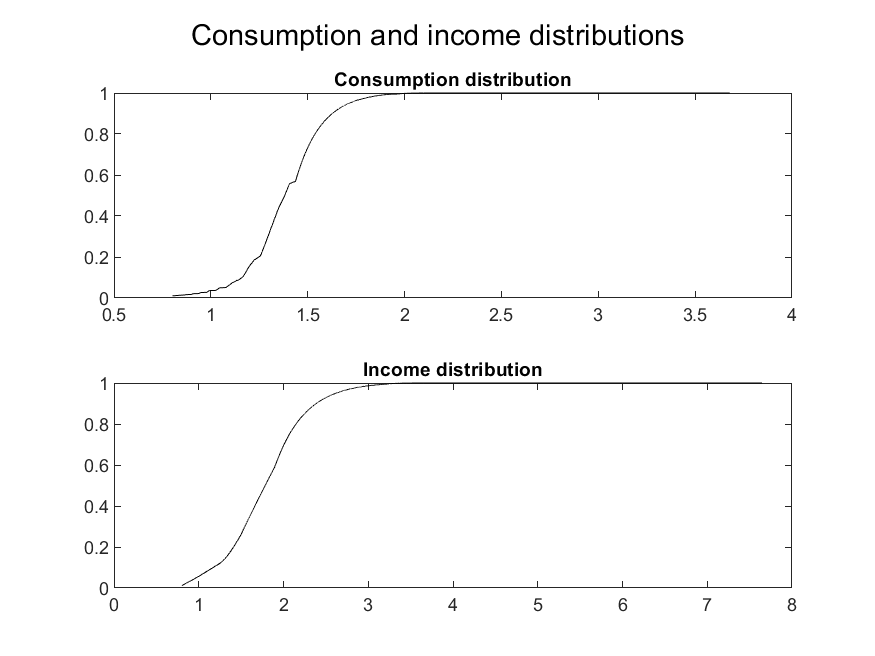
\includegraphics{dis}

Above we can see the distributions for consumption and income, as represented by their CDFs. The consumption distribution has a much tighter spread than the income distribution, with the vast majority of the population mass consuming between 1 and 1.7 units of the consumption good, while the majority of the population mass has an income between 1 and 2.5 units of the consumption good. This makes sense, as individuals make their asset savings choice to smooth consumption, so income spread should be wider than the consumption spread. Below, we will observe the change in the distribution from changing the lower bound on assets.

\subsection{Part C}

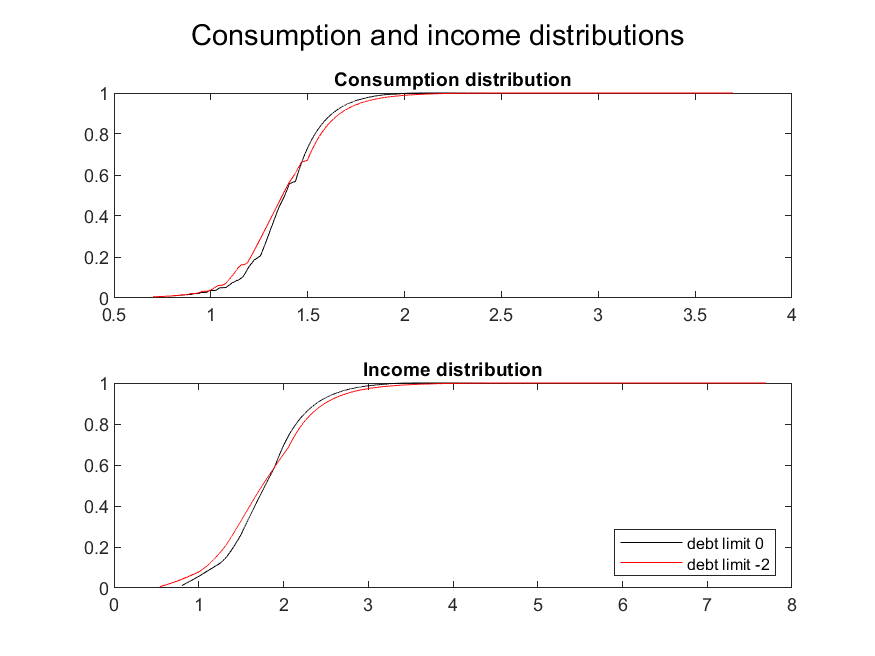
\includegraphics{comp}

With the lower debt limit, the consumption and income distributions widen. Individuals can get into debt, which they could not before, and if they are continually unlucky with respect to their labor draws, they will go into debt until they hit the lower bound, and if they hit the lower bound then they will be able to afford even less of the consumption good than before, should they continue to be unlucky in their draws. The result is a wider spread in both consumption and income. Below we compare the equilibrium variables in the debt equilibrium with those in Part A.

\begin{center}
R2 & 0.552 & 0.622 & 0.407 \\ 
N & 28 & 29 & 26 \\ 

\end{center}

We see, from the table above, that capital levels fall in the debt equilibrium. Further, the wage falls as labor is less productive with a lower capital level. Finally, the interest rate rises as the interest rate is determined by the derivative of output with respect to capital, which is decreasing in capital.

\section{Question 2}
\subsection{Part A}
Our bellman equation takes the following form:
\begin{align*}
V(k,z) &= \max_{k'} \frac{(zk^{0.35}+(1-\delta)k - k')^{1-\gamma}}{1-\gamma} + \beta\sum_{i=1}^n V(k',z_i)P(z' = z_i|z)
\end{align*}
 We solve this computationally, and compare to our results from before.

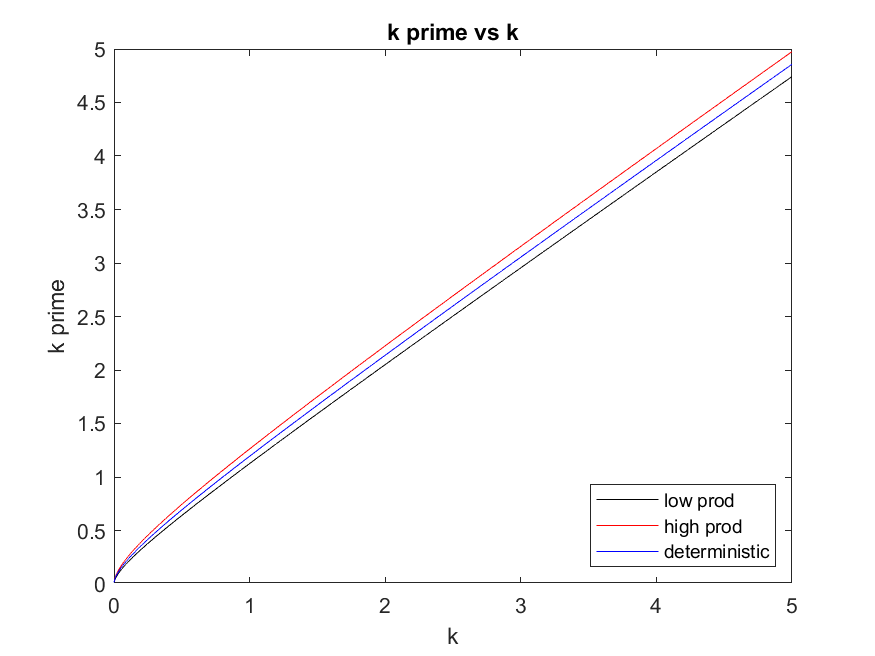
\includegraphics{q2k}

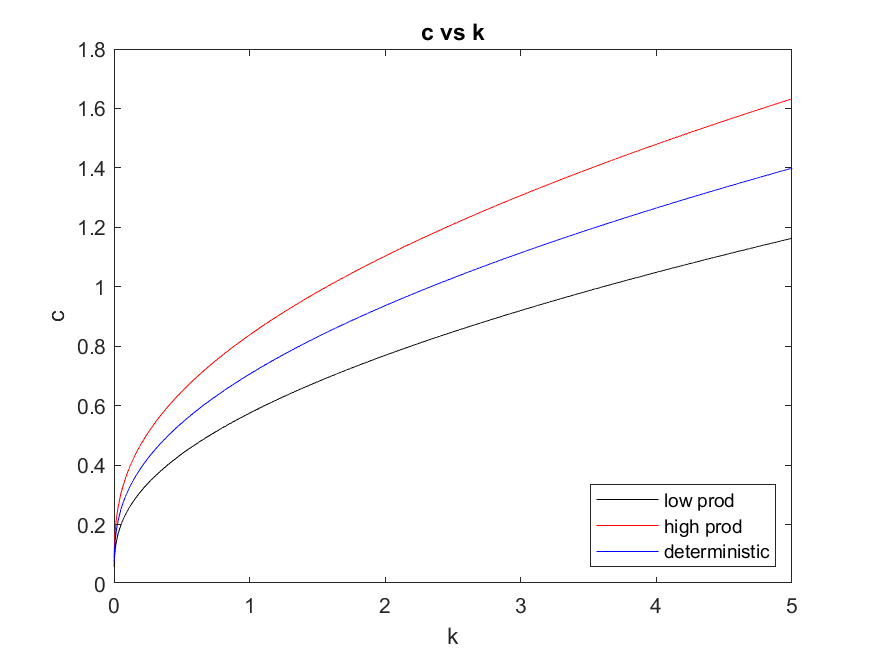
\includegraphics{q2c}

The above plots show that the consumption levels of the high and low equilibrium are, as expected, above and below the original equilibrium. A similar story holds for capital.

\subsection{Part B}
We start with an initial distribution of capital levels and, after a burn-in period, track capital, output, consumption, investment, wages, and interest rates over time. I ran the simulation 100000 times with a burn-in of 10000 draws (for a total of 110000 draws) from an initial uniform distribution over the states, and the averages of the variables of interest appeared to converge by the end of the simulation period, specifically numerical results are unchanged to the fourth decimal point from when the number of draws is reduced by a factor of 10. Results and comparison to the deterministic model are below.

\begin{center}
\begin{tabular}{lll}
& Deterministic & Simulation \\ 
\hline 
Capital & 3.5841 & 3.6302 \\ 
Output & 1.5633 & 1.5653 \\ 
Consumption & 1.2049 & 1.2182 \\ 
Investment & 0.35841 & 0.36302 \\ 
wages & 1.0161 & 1.0174 \\ 
interest rates & 0.15266 & 0.15373 \\ 
\hline 
\end{tabular}
\end{center}

On average, consumption in the stochastic case is higher than the deterministic case. This is due to capital being higher on average in the stochastic case compared to the deterministic case. Individuals are saving more to hedge against the bad productivity draws that may come in the future, and therefore end up consuming more on average as they are wealthier on average.

\subsection{Part C}
We calculate the volatilities and correlations as requested, reported below.

\begin{center}
\begin{tabular}{ll}
& Simulation \\ 
\hline 
Consumption Volatility & 0.26209 \\ 
Output Volatility & 0.092208 \\ 
Investment Volatility & 0.10719 \\ 
C-Y Correlation & 0.71852 \\ 
r-Y Correlation & -0.99692 \\ 
\hline 
\end{tabular}
\end{center}

We can see that consumption's volatility is high, much higher than output or investment volatility (reported volatility measures are the standard deviations of the simulated time series). Output and investment volatilities are roughly similar.

We see a high and positive correlation between output and consumption. This makes sense as more output implies a higher budget, and therefore higher consumption. The near-perfect negative correlation between the interest rate and output is very interesting. In this model, this is caused by the fact that both the interest rate and output are exactly determined by the capital level, so for small changes in capital levels the relationships between both the interest rate and output with capital levels are approximately linear, and therefore there is an approximate linear mapping between the interest rate and output (i.e. first-order taylor approximations mapping capital to the interest rate and capital to output yield a linear mapping between the interest rate and output). The near-unit magnitude of the correlation implies that the capital level is fluctuating by a sufficiently small amount over time for the approximate linear mappings between these variables to be very accurate.

\section{Question 3}
\subsection{Part A}
The household's Bellman equation is the following:
\begin{align*}
V(k,z) &= \max_{k'} u(c) + \beta \int V(k',z')P(z',z)\\
\text{s.t. } c+k' - (1-\delta)k &= (1-\tau)(w + rk) + T
\end{align*}
\begin{align}
\Rightarrow V(k,z) &= \max_{k'} u((1-\tau)(w + rk) + T + (1-\delta)k - k') + \beta \int V(k',z')P(z',z) \label{eqn:hh}
\end{align}

Firms maximize production (note: no disutility from working implies labor supply, and therefore demand, will be 1). Define $f(k):= F(k,1)$.

\begin{align}
\max_{k^d} zf(k^d) - w - rk^d \label{eqn:firm}
\end{align}

The government's budget constraint is $\tau(w+rk) = T$.

Market clearing implies the following:

\begin{align}
k^d &= k\label{eqn:k}\\
zf(k^d) &= c+ k' - (1-\delta)k\label{eqn:c}
\end{align}

The competitive equilibrium is a set of $\{w_t,r_t\}_{t=0}^{\infty}$ and allocations $\{c_t,k_t, k_t^d\}$ such that households optimize (\ref{eqn:hh}), firms optimize (\ref{eqn:firm}), the government budget constraint holds, and capital and goods markets clear (\ref{eqn:k},\ref{eqn:c}).

\subsection{Part B}
We can solve the household's problem by taking first order conditions and envelope conditions:
\begin{align*}
u'(c)&= \beta E[V'(k',z')|z]\\
V'(k,z) &= u'(c)((1-\tau)r + (1-\delta))\\
\end{align*}
\begin{align}
\Rightarrow u'(c)&= \beta E[u'(c')((1-\tau)r' + (1-\delta))|z] \label{eqn:euler}
\end{align}

Our law of motion of capital supply must satisfy the euler equation (\ref{eqn:euler}).

\subsection{Part C}
We now continue to solve the problem.

The firm's optimization conditions set $r = zf'(k^d)$, zero profits set $w = zf(k^d) - rk^d$, and market clearing in the capital market implies $k^d = k$. We then have the following:

\begin{align}
 u'(c)&= \beta E[u'(c')((1-\tau)z'f'(k') + (1-\delta))|z] \label{eqn:eq1}\\
k' &= zf(k) - c + (1-\delta)k\label{eqn:eq2}
\end{align}

The above equations (\ref{eqn:eq1}),(\ref{eqn:eq2}) form a law of motion consumption and capital, and thus are our functional equations for which the consumption and capital accumulation must satisfy.
\subsection{Part D}
Now let $\delta = 1.$ Our competitive equilibrium conditions reduce to the following:

\begin{align}
 1&= E[\beta\frac{u'(c')}{u'(c)}((1-\tau)z'f'(k'))|z] \label{eqn:eq1}\\
k' &= zf(k) - c \label{eqn:eq2}
\end{align}

The social planner chooses consumption and capital to maximize consumption:
\begin{align*}
&\max_{\{c_t,k_t\}_{t=0}^{\infty}} \sum_{t=0}^{\infty}\beta^t u(c)\\
&\text{s.t. } c_t+k_{t+1}  = z_tf(k_t)\\
\Rightarrow &\max_{\{k_t\}_{t=0}^{\infty}} \sum_{t=0}^{\infty} \beta^{t} u( z_tf(k_t) - k_{t+1})\\
\Rightarrow &E[\beta^t u'( c_t)z_tf'(k_t)|z_{t-1}] = E[\beta^{t-1} u'(c_{t-1})|z_{t-1}]
\end{align*}
Rearranging and dropping the time subscripts, we find the following:
\begin{align}
\Rightarrow 1 &= E\left[\beta\frac{u'(c')}{u'(c)}z'f'(k')|z \right], \label{eqn:spc}\\
k' &= zf(k) - c.\label{eqn:spk}
\end{align}

We can clearly see that our functional equations across the social planner's solution (\ref{eqn:spc}),(\ref{eqn:spk}) and competitive equilibrium (\ref{eqn:eq1}),(\ref{eqn:eq2}) are identical except for the distortionary $(1-\tau)$ term in the discount factor of the competitive equilibrium. Essentially, the distortionary taxes make the households consume more and save less, as the taxes reduce their returns to saving.

\section{Question 4}
Epstein-Zin preferences take the following form (note the correction here to the typo in the problem set):
\begin{align*}
V_t &= \left( (1-\beta) c_t^{1-\rho} + \beta(E_tV_{t+1}^{1-\alpha})^{\frac{1-\rho}{1-\alpha}} \right)^{\frac{1}{1-\rho}}
\end{align*}
\subsection{Part A}
Let $\alpha = \rho$.
\begin{align*}
V_t &= \left( (1-\beta) c_t^{1-\rho} + \beta(E_tV_t^{1-\alpha})^{\frac{1-\rho}{1-\alpha}} \right)^{\frac{1}{1-\rho}}\\
&= \left( (1-\beta) c_t^{1-\rho} + \beta(E_tV_t^{1-\rho}) \right)^{\frac{1}{1-\rho}}
\end{align*}
This is equivalent to the following value function:
\begin{align*}
W_t &= (1-\beta) c_t^{1-\rho} + \beta(E_tW_t),
\end{align*}
where $W_t = V_t^{1-\rho}$ which is the value equation representation of power utility.
\subsection{Part B}
The risk aversion for static gamples here is represented by the $\alpha$ parameter on consumption, and $1/\rho$ is the inverse of the intertemporal elasticity of substitution.
\subsection{Part C}
\begin{align*}
\frac{\partial V_t}{\partial V_{t+1}} &= \frac{1}{1-\rho}V_t^{\rho}\frac{1-\rho}{1-\alpha}\beta (E_tV_{t+1}^{1-\alpha})^{\frac{\alpha-\rho}{1-\alpha}}(1-\alpha)E_tV_{t+1}^{-\alpha} \\
&= \beta V_t^{\rho}  (E_tV_{t+1}^{1-\alpha})^{\frac{\alpha-\rho}{1-\alpha}} E_tV_{t+1}^{-\alpha}\\
\frac{\partial V_{t}}{\partial c_{t}} &=\frac{1}{1-\rho}V_t^{\rho}((1-\beta)(1-\rho)c_t^{-\rho}) \\
\Rightarrow S_t &= \frac{\frac{\partial V_t}{\partial V_{t+1}}\frac{\partial V_{t+1}}{\partial c_{t+1}} }{\frac{\partial V_{t}}{\partial c_{t}} }\\
&= \frac{ \beta V_t^{\rho}  (E_tV_{t+1}^{1-\alpha})^{\frac{\alpha-\rho}{1-\alpha}} E_tV_{t+1}^{-\alpha}V_{t+1}^{\rho}c_{t+1}^{-\rho} }{V_t^{\rho}c_t^{-\rho} }\\
&= \frac{ \beta  (E_t[V_{t+1}^{1-\alpha}])^{\frac{\alpha-\rho}{1-\alpha}} E_t[V_{t+1}^{-\alpha}]V_{t+1}^{\rho}c_{t+1}^{-\rho} }{c_t^{-\rho} } 
\end{align*}
\subsection{Part A'}
Our endowment process follows an iid growth rate. Let $s_t$ be the fruit from our Lucas tree, and in equilibrium $s_t = c_t$. Then, $c_{t+1}/c_t = g+\sigma_c\epsilon_{t+1}$ where $\epsilon_t\sim N(0,1).$ We conjecture that our prices are a function of s, $p = p(s)$
Our Bellman equation takes the following form:
\begin{align*}
V([p(s) +s]a) &= \max_{c,a'} ((1-\beta) c^{1-\rho} + \beta (E [ (V([p(s') + s']a'))^{1-\alpha} ])^{\frac{1-\rho}{1-\alpha}})^{\frac{1}{1-\rho}}\\
&\text{s.t. } c+p(s)a' = (p(s)+s)a\\
\Rightarrow V([p(s) +s]a) &=\max_{a'}  ((1-\beta) ((p(s) + s)a - p(s)a')^{1-\rho} + \beta (E [ (V([p(s') + s']a'))^{1-\alpha} ])^{\frac{1-\rho}{1-\alpha}})^{\frac{1}{1-\rho}}
\end{align*}

%\begin{align*}
%V(c) &= \max_{c} ((1-\beta) c^{1-\rho} + \beta (E [ (V(c')^{1-\alpha} ])^{\frac{1-\rho}{1-\alpha}})^{\frac{1}{1-\rho}}
%\end{align*}
\subsection{Part B'}
The recursive competitive equilibrium is a set of prices $\{p(c_t)\}_{t=0}^{\infty}$ and allocations $\{c_t,a_t \}$ such that agents follow their bellman equation and markets clear ($a_t = 1, c_t = s_t$).
\subsection{Part C'}
%\begin{align*}
% \frac{1}{1-\rho}V^{\rho}((1-\beta)(1-\rho)c^{-\rho}p(s) +\beta\frac{1-\rho}{1-\alpha}(E[(V([p(s') + s']a'))])^{\frac{\rho - \alpha}{1-\alpha}}
%\end{align*}
We guess and verify that our value function can be written $V(c) = vc$ for some constant $v$.
\begin{align*}
vc&= \max_{a'} ((1-\beta) c^{1-\rho} + \beta (E [ v^{1-\alpha}c'^{1-\alpha}|c ])^{\frac{1-\rho}{1-\alpha}})^{\frac{1}{1-\rho}}\\
&=( (1-\beta) c^{1-\rho} + \beta(E [ v^{1-\alpha}(c)^{1-\alpha}(g+\sigma_c \epsilon ')^{1-\alpha} ])^{\frac{1-\rho}{1-\alpha}})^{\frac{1}{1-\rho}}\\
\Rightarrow v &= ( (1-\beta)  + v^{1-\rho}\beta(E [ (g+\sigma_c \epsilon ')^{1-\alpha} ])^{\frac{1-\rho}{1-\alpha}})^{\frac{1}{1-\rho}}
\end{align*}

$v$ solves this one equation in one unknown, which is not a function of $c$ and thus is a constant given a parameterization.

From our expression above for $S_t$,

\begin{align*}
log(S_t) &= log(\beta)+\frac{\alpha - \rho}{1-\alpha}log(E_t[(vc_{t+1})^{1-\alpha}]) \\
&+log(E_t[(vc_{t+1})^{-\alpha}]) + \rho log(v) + \rho log(c_t) - \rho log(c_t) + \rho log(c_{t+1})\\
&=log(\beta)+\frac{\alpha - \rho}{1-\alpha}log(E_t[(vc_{t+1})^{1-\alpha}]) +log(E_t[(vc_{t+1})^{-\alpha}]) + \rho log(v) + \rho log(c_{t+1})
\end{align*} 
\subsection{Part D'}
We know that the price of a bond, $P^b(c) = E[mx]$ where $m$ is the stochastic discount factor and $x$ is the payoff of the bond. The risk-free payoff is always $1$ and we solved for $m = S_t$ above, so we can plug in:
\begin{align*}
P^f(c_t) &= E_t[S_t] \\
R^f(c_t) &= \frac{1}{E_t[S_t]}.
\end{align*}
In the risk-free case, the risk-free bond price is $\frac{1}{E[m]}$, where $m$ is the stochastic discount factor. So, the form of the expression written in this form is the same, in terms of its relationship to the stochastic discount factor. However, in the CRRA case the stochastic discount factor takes a different form $\left( \beta\frac{u'(c')}{u'(c)} \right)$ which is far different from the expression we solved for $S_t$ before.
\subsection{Part E'}
We know our pricing kernel and can price the bonds as $P^l(c_t) = E[S_tx]$, where $x$ is the payoff of the claim to the tree:
\begin{align*}
P^l(c_t) &= E_t[S_t (P^l(c_{t+1}) +c_{t+1})|c] \\
&=  E_t[S_t (P^l(c_t(g+\sigma_c\epsilon_{t+1})) +c_t(g+\sigma_c\epsilon_{t+1}))]\\
R^l(c_t) &= \frac{1}{P^{l}(c_t)}.
\end{align*}
As before, the structure of the bond price expression is functionally the same as in the CRRA case, but with a much different formulation for the stochastic discount factor.
\end{document}
